\documentclass[titlepage,a4paper]{article}

\usepackage{a4wide}
\usepackage[colorlinks=true,linkcolor=black,urlcolor=blue,bookmarksopen=true]{hyperref}
\usepackage{bookmark}
\usepackage{fancyhdr}
\usepackage[spanish]{babel}
\usepackage[utf8]{inputenc}
\usepackage[T1]{fontenc}
\usepackage{graphicx}
\usepackage{float}

\pagestyle{fancy} % Encabezado y pie de página
\fancyhf{}
\fancyhead[L]{TP2J - AlgoPoly}
\fancyhead[R]{Algoritmos y Programación III - FIUBA}
\renewcommand{\headrulewidth}{0.4pt}
\fancyfoot[C]{\thepage}
\renewcommand{\footrulewidth}{0.4pt}

\begin{document}
\begin{titlepage} % Carátula
	\hfill
\includegraphics[width=6cm]{fiuba.jpg}
    \centering
    \vfill
    \Huge \textbf{Trabajo Práctico 2 — Java}
    \vskip2cm
    \Large [7507/9502] Algoritmos y Programación III\\
    Curso 1 \\ % Curso 1 para el de la tarde y 2 para el de la noche
    Segundo cuatrimestre de 2017 
    \vfill
    \begin{tabular}{|l|c|r|}
	\hline
    Alumno & Padrón & Mail\\
	\hline
	Victoria Zambianchi & 98570 & viky.zambi@gmail.com\\
	\hline
    Federico del Mazo & 100029 & delmazofederico@gmail.com\\
	\hline
    Nicole Raveszani & 101031 & nraveszani@gmail.com\\
	\hline
    Florencia Rodríguez & 100033 & florrr1997@gmail.com\\
	\hline
	\end{tabular}
    \vfill
    \vfill
    
    
\end{titlepage}

\tableofcontents % Índice general
\newpage

\section{Introducción}\label{sec:intro}
El presente informe reune la documentación para la primera entrega del trabajo práctico número 2 en Java "AlgoPoly".

\section{Supuestos}\label{sec:supuestos}
% Deberá contener explicaciones de cada uno de los supuestos que el alumno haya tenido que adoptar a partir de situaciones que no estén contempladas en la especificación.
\begin{description}
\item[Avance y retroceso dinámico] Estas dos clases devuelven uno que hace referencia a la cantidad de movimientos que debe realizar elk jugador para llegar a su posición final. uponemos que las  cuentas dadas para los distintos rangos de resultado de dado no puede ser negativos. Por ejemplo, que la cantidad de propiedades siempre será menor a 11, y de esta manera, en avance dinámico nunca se devolvera un número negativo, La misma lógica se aplico en retroceso dinámico.
\item[Barrio] El jugador es libre de decidir que barrios comprar y si queire contruir casas u hoteles. El juego jamas le dejara contruir un hotel a un jugador que no tenga los barrios y edificaciones necesarias


\end{description}

\section{Modelo de dominio}\label{sec:modelo}

Paquete Modelo:

% Explicación concisa del diseño general del trabajo.
\begin{itemize}
\item 
Clase Jugador: representa a un jugador de AlgoPoly. Posee un nombre a elección del usuario y comienza el juego con determinado capital. Puede adquirir propiedades y edificar sobre las mismas en caso de tener el capital suficiente. Además, según en qué casillero se encuentre, el comportamiento del mismo puede afectar su capital o su capacidad de movimiento en los siguientes turnos.
\end{itemize}

\begin{itemize}
\item 
Clase Municipio: representa una entidad administrativa que se encarga de conocer y actualizar los propietarios y la cantidad de edificaciones (en caso de ser un barrio) de aquellas clases que implementen la interfaz Propiedad, cuando los jugadores ejecuten acciones sobre alguna propiedad. Al poseer una base de estos datos, puede decir quien es el propietario de cada propiedad, ceder la misma al banco de ser necesario, si un jugador es capaz de edificar en un barrio una casa o un hotel.
\end{itemize}

\begin{itemize}
\item 
Clase Tablero: representa el tablero de juego AlgoPoly. El tablero se llena al ser instanciado por todos los casilleros correspondientes al juego. Se encarga de seleccionar la posición siguiente de cada jugador basándose en su posición actual y en el número que salió en la tirada de dados.
\end{itemize}

\begin{itemize}
\item 
Clase Turno: representa un turno correspondiente a un jugador de AlgoPoly. En caso de que el jugador pueda moverse, le solicita al tablero el casillero siguiente al jugador y se lo asigna.
\end{itemize}

\begin{itemize}
\item 
Clase Dados: se instancia con dos números generados al azar del 1 al 6 y puede devolver la suma o si ambos números son idénticos.
\end{itemize}

\begin{itemize}
\item
Clase Edificacion: representa una construccion que puede hacer una propiedad. Posee su su costo de edificación y el alquiler que otorga.
\end{itemize}

\begin{itemize}
\item 
Interfaz Estado: la interfaz obliga a aquellos que la implementan (las clases Libre y Preso) a devolver si el movimiento es posible y a habilitar el movimiento.
\end{itemize}

\begin{itemize}
\item 
Clase Libre: representa que el jugador es libre de moverse.
\end{itemize}

\begin{itemize}
\item 
Clase Preso: representa que el jugador se encuentra preso en la Carcel. Para moverse es necesario que el jugador haya jugado 3 turnos o haber pagado la fianza. Para habilitar el movimiento se le solicita la fianza al jugador
\end{itemize}

Paquete Casilleros:

\begin{itemize}
\item 
Interfaz Casillero: toda clase que la implementa es la representación de una casilla. Esta interfaz las obliga a tener los métodos accionAlCaer(), que es la acción que se ejecuta cuando un jugador cae en determinado casillero, nombre() y color() que son necesarios en métodos de otras clases.
\end{itemize}

\begin{itemize}
\item 
Interfaz Propiedades: toda clase que la implementa es la representación de una propiedad, con esto nos referimos a aquellos casilleros que tienen la particularidad de poder ser adquiridos por un jugador y aumentar su capital bajo ciertas condiciones. Una propiedad puede tratarse tanto de un barrio como un servicio.
\end{itemize}

\begin{itemize}
\item 
Clase Barrio: representa a un barrio del juego AlgoPoly. Puede ser comprado y vendido por un jugador, el propietario puede edificar construcciones y al caer un jugador que no es el propietario debe pagar un alquiler a quien lo sea.
\end{itemize}

\begin{itemize}
\item 
Clase BarrioDoble: posee el mismo comportamiento que la clase Barrio, a diferencia de que se puede reemplazar a las casas por un hotel unicamente si el jugador es propietario ademas del barrio doble requerido.
\end{itemize}

\begin{itemize}
\item 
Clase Servicio: representa un servicio del juego AlgoPoly. Al igual que el barrio, puede ser comprado y vendido por un jugador. Si un jugador que no es el propietario cae en una instancia de este casillero, se le cobra un costo de servicio igual al costo original del servicio (que depende de si el jugador propietario posee o no la propiedad doble correspondiente) multiplicado por el numero de dados que saco.
\end{itemize}

\begin{itemize}
\item 
Clase Policia: representa a la policia del juego AlgoPoly. Cuando el jugador cae en Policia lo envia a la Carcel.
\end{itemize}

\begin{itemize}
\item 
Clase Carcel: representa una cárcel del juego AlgoPoly. Al caer en ella, el jugador es incapaz de moverse hasta que no se cumplan ciertas condiciones.
\end{itemize}

\begin{itemize}
\item 
Clase ImpuestoAlLujo: cuando un jugador cae en ella, lo único que hace es quitarle un %10 su capital.
\end{itemize}

\begin{itemize}
\item 
Clase Quini6: representa una lotería. Al caer en ella, el jugador puede o no recibir dinero, depende de cuantas veces cayó previamente. La primera vez recibe 50000, la segunda 30000 y para el resto del juego ya no recibe dinero.
\end{itemize}

\begin{itemize}
\item 
Clase Salida: donde comienzan todos los jugadores. No tiene efecto alguno.
\end{itemize}
\begin{itemize}
\item 
Clase Dinamismo: esta clase abstracta es  la representación de un casillero que posee la particularidad de ser dinámica. Con esto nos referimos a que cuando un jugador cae en estas casillas  dinámicas, se  establece un comportamiento especifico, el cual hace que el jugador pueda avanzar o retroceder en el tablero.
\end{itemize}
\begin{itemize}
\item 
Clase AvanceDinamico: representa a un casillero que tiene la cualidad  especial de hacer avanzar al jugador en el tablero  dependiendo del número de dados que saco. Si el jugador en su partida caen en este casillero entonces debera avancar cuanto se lo diga.
\end{itemize}
\begin{itemize}
\item 
Clase RetrocesoDinamico: representa a un casillero que tiene la cualidad especial de hacer retroceder al jugador en el tablero dependiendo del numero de dado. Si el jugador en su partida cae en este casillero entonces debera retroceder cuanto se lo diga.  
\end{itemize}

Paquete Vista: 
\begin{itemize}
\item 
Clase ContenerdorEntrada :  visualización de la presentación del juego dónde los tres jugadores pueden elegir sus nombres y el color de sus piezas, los nombre ingresados son luego utilizados para iniciar el juego.
\end{itemize}
\begin{itemize}
\item 
Clase ContenedorPrincipal : visualización del juego, este posee al tablero, la consola dónde se puede ver toda acción desarrollada, y por último a la derecha los botones que puede utilizar el jugador.
\end{itemize}
\begin{itemize}
\item 
Posición : controla la siguiente posición del jugador, tal que devuelve la nueva ubicación de este. También se utiliza al presentar el tablero, siendo esta una manera más automática de formarlo.
\end{itemize}
\begin{itemize}
\item 
VistaJugador : visualización del jugador, representado por un círculo del color elegido en el contenedor de entrada. Conoce su posición y se mueve debido a Posición.
\end{itemize}
\begin{itemize}
\item 
Paquete Controladores: 
El paquete controladores posee por una parte el conjunto de todos los botones manejados en el juego:
-Tirar Dados
-Comprar
-Vender
-Edificar casa
-Edificar Hotel
-Pagar Fianza ( para poder salir de la cárcel)
-Mute (para poder silenciar la música de fondo)

Siempre que se clickea un botón, es decir, se activa un handler de eventos, el visor y la vista del tablero se actualiza para poder estar al día con las últimas acciones del usuario. Por ejemplo, el pagar la fianza hace que el visor del usuario informe que ya no está más preso. Esto se logra en gran parte gracias a que el controlador de turnos es una clase Singleton.
 \end{itemize}
Y por otro lado:
\begin{itemize}
\item
ControladorDeTurno : esta es una clase Singleton, ya que hay solamente un juego en desarrollo y por ejemplo, los botones necesitan en todo momento saber quién lo está seleccionando, presuponiendo que lo toca quién esté jugando en el momento.
\end{itemize}
\begin{itemize}
\item 
EntradaUsuario : guarda toda información ingresada por el usuario en la entrada del juego.
\end{itemize}

\section{Detalles de implementación}\label{sec:detallesdeimplementacion}

Paquete Modelo:

\begin{itemize}
\item 
Clase Jugador: es instanciado con un capital total de 100000, su casillero actual es null y su estado es una nueva instancia de libre. Recibe el nombre por parámetro. Todos los métodos relacionados con las propiedades, ya sean comprar, vender al banco, entre las más importantes, acceden al Municipio que se encarga de actualizar los respectivos datos. Para saber si el jugador es capaz de moverse, se debe verificar si su estado es una instancia de Libre o Preso. En el primer caso, el jugador es libre de moverse y puede lanzar los dados, en el caso contrario debe permanecer en esa casilla hasta que se ejecuten las acciones necesarias. Por ejemplo, si el jugador cayó en Carcel, es incapaz de moverse hasta que no pasen los días necesarios o se pague la fianza. Para lograr esto se uso el patron de dise;o State ya que consideramos necesario que el comportamiento del jugador cambiara segun si puede o no moverse.
\end{itemize}

\begin{itemize}
\item 
Clase Municipio: el municipio fue creado como un Singleton debido a que necesitábamos un único lugar donde almacenar y actualizar la información correspondiente a las propiedades, el cual pudiera ser accedido por instancias de Jugador, tanto por Barrio y Servicio, por los controladores correspondientes a los botones y por Visor. Al usar un Singleton, pudimos garantizar un único punto de acceso a esa base de datos y encapsular la responsabilidad de conocer, actualizar y otorgar permisos para los métodos relacionados a las propiedades y sus propietarios.

	Con respecto al resto de la implementación, posee cinco diccionarios de los cuales 3 son actualizados al comienzo con la información de un archivo de texto y el resto se van actualizando a medida que se requiere su uso con los datos que reciben.
    
	El diccionario propietarios: posee como clave el nombre de la propiedad y como valor la instancia del jugador al que le pertenece.
    
	El diccionario hermano: posee como clave el el nombre de la propiedad y su propiedad hermana.
    
	El diccionario alquilerServicio: posee como clave el nombre del servicio y una dupla que contiene en primer lugar el servicio que se compra al tener la propiedad y en segundo lugar, el servicio que se cobra al tener la propiedad hermana.
    
	El diccionario jugadorPropiedades: posee como clave el nombre del jugador y una lista de todas las instancias de propiedades que le pertenecen.
    
	El diccionario cantEdificaciones: posee como clave el nombre de la propiedad y la cantidad de edificaciones que tiene hasta el momento.
\end{itemize}

\begin{itemize}
\item 
Clase Tablero: al igual que el Municipio, el tablero fue creado como un Singleton debido a que varias clases necesitan cambiar la posición del jugador y para encapsular ese comportamiento decidimos crear una única clase que pudiera ser accedida globalmente. Además, facilitó bastante la lectura del código ya que las clases no necesitan recibir al tablero como parámetro. Posee una lista en la que se almacenan todas las instancias creadas de los barrios.
\end{itemize}

Paquete Casilleros (todos implementan Casillero):

\begin{itemize}
\item 
Clase Barrio: posee atributos para el nombre del propietario, el nombre del barrio, su costo, la lista de casas que se hayan edificadas, el alquiler actual (que se actualiza con cada casa edificada) y el alquiler original (el alquiler con el que se creo el barrio), el valor del mercado (la cantidad de dinero que recibe el jugador al venderlo). Los metodos relacionados a comprar, vender y edificar se encargan de restarle o sumarle la cantidad correspondiente al capital del jugador y actualizar los datos en el municipio.
\end{itemize}

\begin{itemize}
\item 
Clase BarrioDoble: hereda de BarrioDoble y puede reemplazar a las casas por un hotel. Para poder edificar un hotel, debe comprobar que el jugador es usuario tanto de este barrio como del otro barrio que corresponde.
\end{itemize}

\begin{itemize}
\item 
Clase Servicio: posee atributos para costo, costo del mercado y nombre. Para calcular el cobro del servicio se verifica el propietario en la Municipalidad.
\end{itemize}

\begin{itemize}
\item 
Clase Carcel: la acción que se ejecuta cuando un jugador cae en este casillero es cambiarle su estado a una nueva instancia de Preso. Esto se puede ver mas detallado en la parte donde se explica la implementación de Jugador.
\end{itemize}
\begin{itemize}
\item 
Clase Dinamismo: esta clase abstracta establece la acción que se va a ejecutar cuando un jugador caiga en el casillero y establece tres métodos abstractos para que sus hijas definan. Asi logrando  que cada casillero sepa como moverse dinámicamente por si sola, logrando evitar codigo repetido. 
\end{itemize}
\begin{itemize}
\item 
Clase AvanceDinamico: esta es una clase que hereda de Dinamismo. En la cual se definen los 3 métodos necesarios para poder calcular a que casillero debe avanzar el jugador dependiendo del número que saco en el dado. La accion que se ejecuta cuando cuando el jugador cae en este casillero dinámico es que avance una cierta cantidad de casilleros más. 
\end{itemize}
\begin{itemize}
\item 
Clase RetrocesoDinamico: esta es una clase que hereda de Dinamismo. En la cual se definen los 3 métodos necesarios para poder calcular a que casillero debe retroceder el jugador dependiendo del número que sacó en el dado. La acción que se ejecuta cuando cuando el jugador cae en este casillero dinámico es que retroceda una cierta cantidad de casilleros más. 
\end{itemize}




\section{Diagramas de clase}\label{sec:diagramasdeclase}

\begin{figure}[H]
\centering
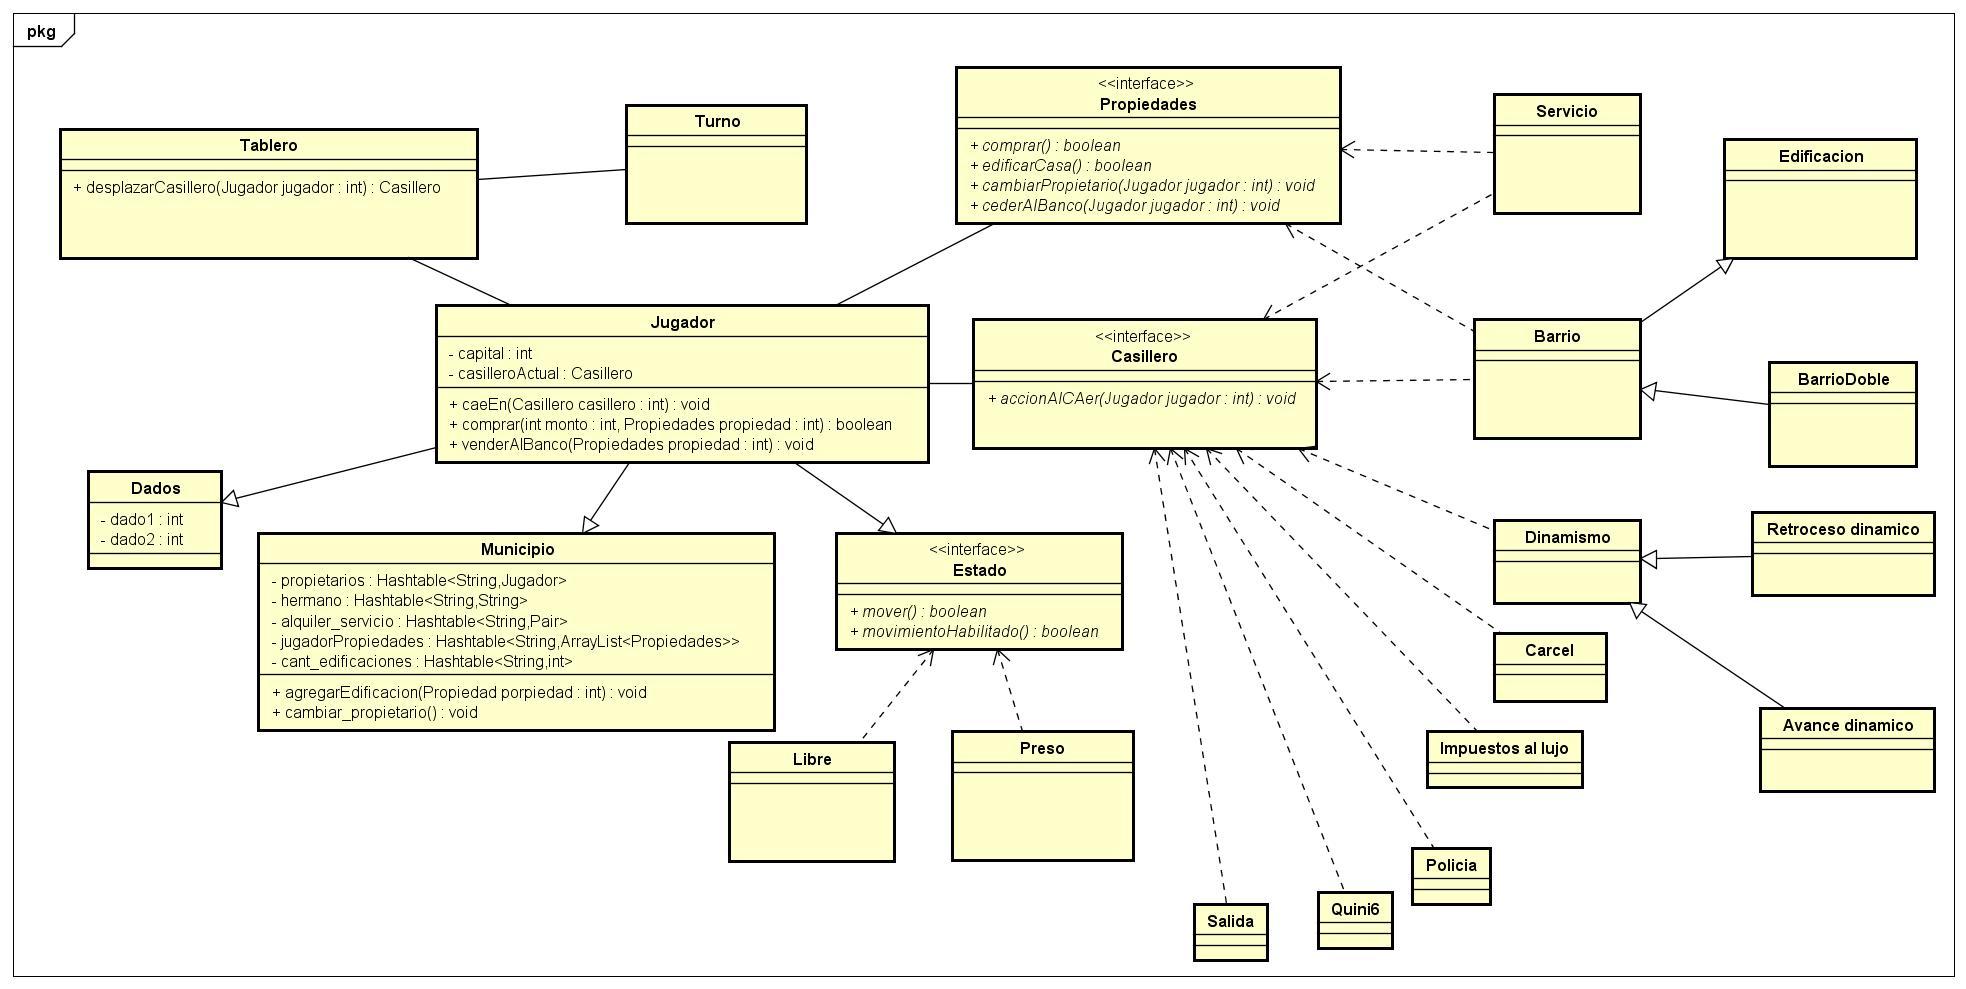
\includegraphics[width=0.8\textwidth]{Class_Diagram0Algopoly2.jpg}
\caption{\label{fig:class01}Diagrama de Clase.}
\end{figure}

\section{Diagramas de Secuencia}\label{sec:diagramadesecuencia}

\begin{figure}[H]
\centering
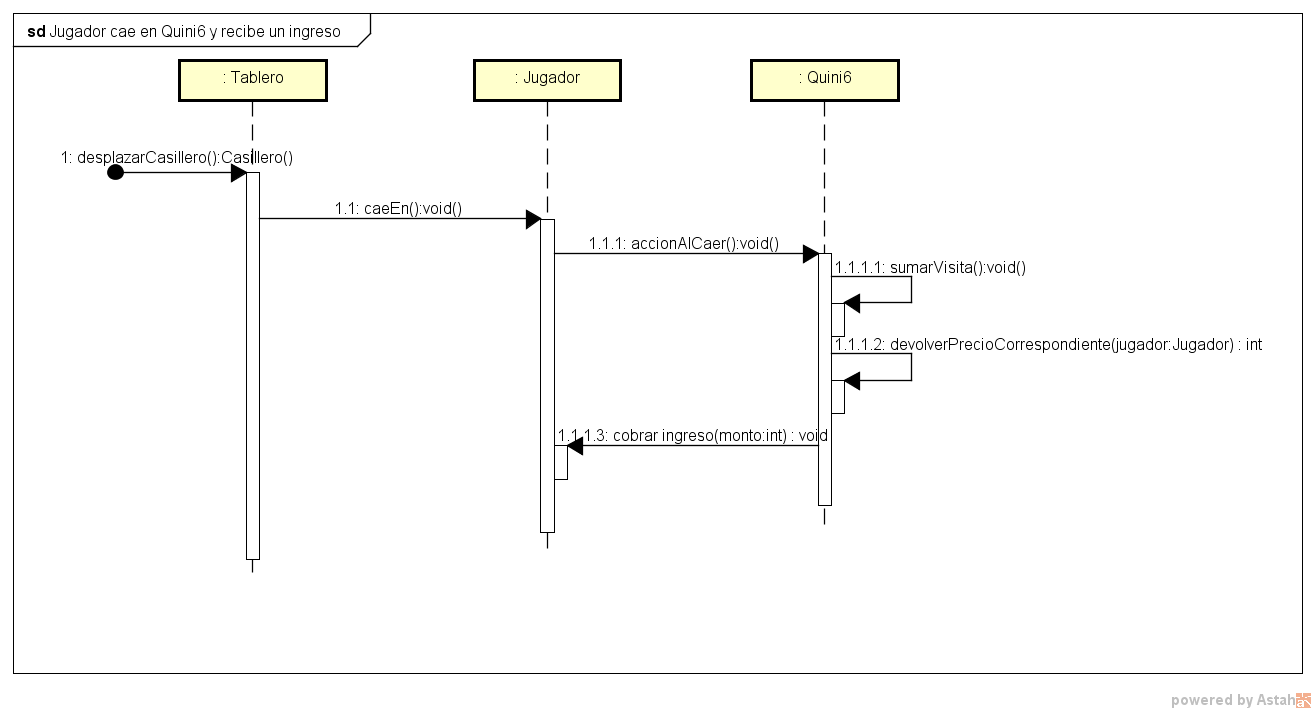
\includegraphics[width=0.8\textwidth]{ALGOPOLY_Jugador_cae_en_Quini6_y_recibe_un_ingreso.png}
\caption{\label{fig:class01}Un jugador cae en Quini6.}
\end{figure}

\begin{figure}[H]
\centering
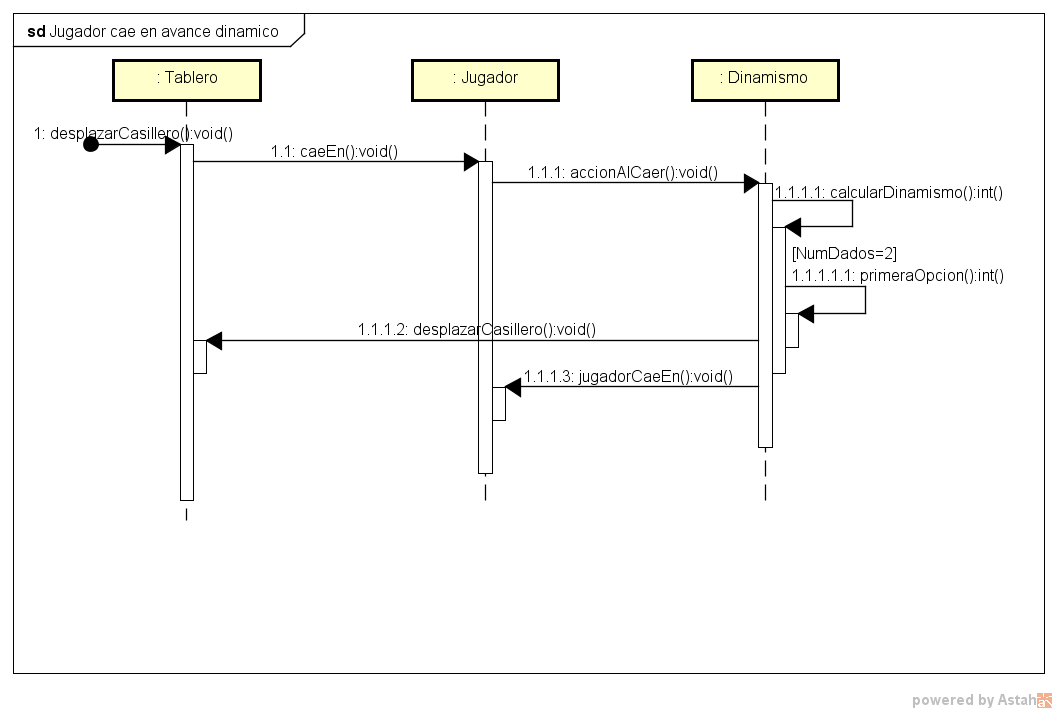
\includegraphics[width=0.8\textwidth]{ALGOPOLY_Jugador_cae_en_avance_dinamico.png}
\caption{\label{fig:class01}Un jugador cae en AvanceDinamico.}
\end{figure}

\begin{figure}[H]
\centering
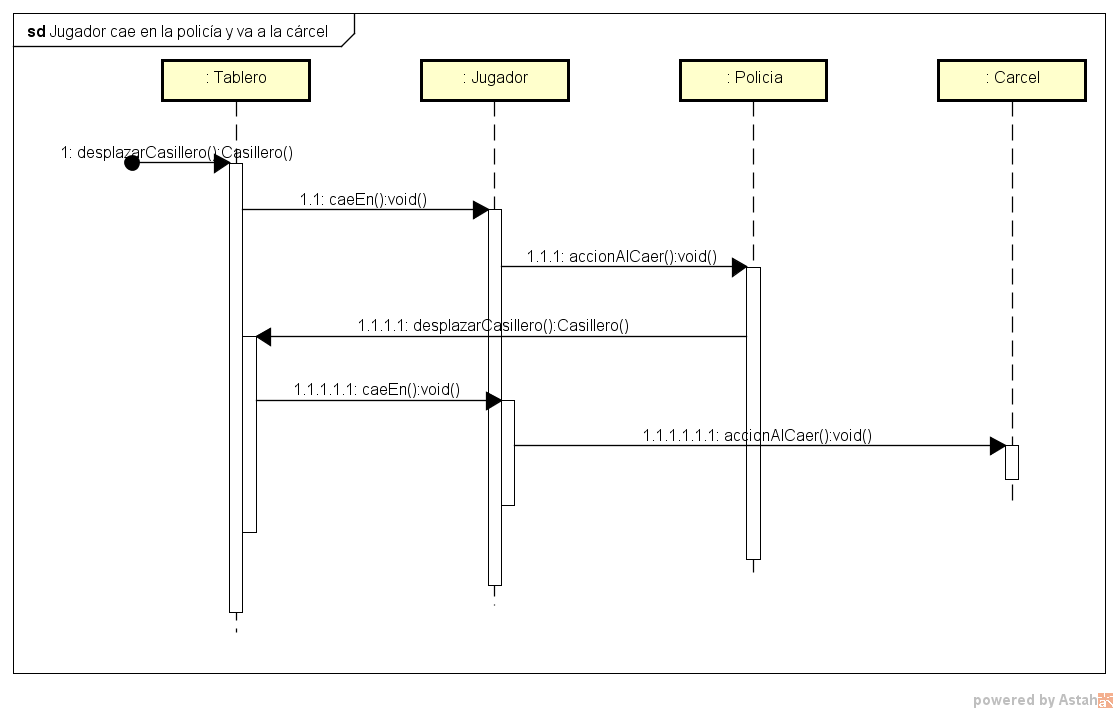
\includegraphics[width=0.8\textwidth]{ALGOPOLY_Jugador_cae_en_la_polic_a_y_va_a_la_c_rcel.png}
\caption{\label{fig:class01}Un jugador cae en Policia.}
\end{figure}

\end{document}